\documentclass[conference]{IEEEtran}
\usepackage[T1]{fontenc}
\usepackage{cite}
\usepackage{amsmath}
\usepackage{graphicx}
\usepackage{booktabs}
\usepackage{tikz}
\usetikzlibrary{arrows.meta,positioning,shapes.geometric}
\usepackage{url}
\usepackage{microtype}

\newcommand{\tbd}{\textbf{TBD}}

\begin{document}

\title{Campus GPT: A Retrieval-Grounded Small Language Model Assistant for Syllabus-Oriented Academic Queries at VTU}

\author{\IEEEauthorblockN{Mallikarjuna P, Vilohitha Sharma, Sayyaf Harif}
\IEEEauthorblockA{Department of Artificial Intelligence and Machine Learning\\
Acharya Institute of Technology, Bengaluru, India\\
USNs: 1AY24AI403, 1AY23AI137, 1AY23AI104}
\and
\IEEEauthorblockN{Dr.\ Vijayashekhar S S}
\IEEEauthorblockA{Professor and Head, Dept.\ of AIML and CSE (DS)\\
Acharya Institute of Technology, Bengaluru, India\\
\textit{Project guide}}}

\maketitle

\begin{abstract}
Students of Visvesvaraya Technological University (VTU) must consult scattered PDFs, slide decks and notes to answer routine questions about syllabus modules, passing rules, grading and attendance. General-purpose chatbots are not aware of the university's scheme and often answer such questions confidently but incorrectly. We present Campus GPT (VTU-SLM-BOT), an academic assistant built around a small instruction-tuned language model, Qwen2.5-1.5B-Instruct, quantized to 4 bits so that it fits a single consumer-grade GPU. Instead of trusting the model's parametric memory, the system routes each query through three paths: an exact fact table for university rules, a structured subject and module knowledge base, and BM25 retrieval over ingested course material with page-level citations. When none of the sources supports an answer, the assistant declines. A parameter-efficient QLoRA fine-tuning stage teaches the model to follow this grounded, cite-or-refuse behaviour. We describe the architecture, the knowledge-base construction pipeline, the fine-tuning recipe and an evaluation protocol with a held-out question set. Quantitative results are reported in Section~\ref{sec:results} once the final training run is complete; this version of the paper contains the protocol and placeholders only.
\end{abstract}

\begin{IEEEkeywords}
small language models, retrieval-augmented generation, educational chatbot, QLoRA, quantization, syllabus question answering
\end{IEEEkeywords}

\section{Introduction}
University students repeatedly ask the same kinds of questions: what topics a module covers, which textbook a course uses, what the minimum marks to pass are, or how a CGPA converts to a percentage. The answers exist in official documents, but those documents are distributed across scheme booklets, per-course syllabus PDFs, regulations and faculty-prepared notes. Cloud-hosted general chatbots can paraphrase this material but are not tied to a particular university's scheme, can hallucinate rules, and require sending student queries to a third party.

Small language models (SLMs) make a different design point possible: a model of roughly one to two billion parameters, quantized to four bits, can run on a single commodity GPU and be adapted cheaply to a narrow domain. The risk is factual unreliability, since small models store little world knowledge. Our central design decision is therefore to treat the model as a language interface over verified sources rather than as a source of truth.

The contributions of this work are:
\begin{itemize}
\item A routed, citation-first architecture for syllabus and regulation question answering that answers university rules from a deterministic fact table and everything else from retrieved documents, with an explicit refusal path.
\item A reproducible knowledge-base pipeline in which every record stores its source URL, retrieval date and a verification flag, so unverified data is never presented as fact.
\item A QLoRA fine-tuning recipe on synthetic question--answer pairs derived from the knowledge base, with a held-out evaluation set kept disjoint from training data.
\item An evaluation protocol covering rule-fact exactness, retrieval hit rate, citation correctness and correct refusal of out-of-scope questions.
\end{itemize}

\section{Related Work}
\textbf{Retrieval-augmented generation.} Lewis et al.\ combine a parametric generator with a non-parametric retriever so that answers are conditioned on retrieved passages and can be traced to them~\cite{lewis2020rag}. We follow this principle but use a lexical retriever, BM25~\cite{robertson2009bm25}, because subject codes and module terminology are exact tokens and the index must be buildable on CPU.

\textbf{Efficient adaptation.} Low-rank adaptation freezes the pretrained weights and trains small rank-decomposition matrices~\cite{hu2022lora}. QLoRA extends this by backpropagating through a 4-bit quantized base model using the NormalFloat (NF4) data type, double quantization and paged optimizers, enabling fine-tuning of billion-parameter models on a single GPU~\cite{dettmers2023qlora}.

\textbf{Small open models.} The Qwen2.5 family provides instruction-tuned models from 0.5B to 72B parameters~\cite{qwen2025}. We use the 1.5B instruction-tuned variant as the generator because it is small enough for a free-tier GPU after quantization.

\textbf{Extractive question answering.} Early prototypes of this project used a distilled BERT model fine-tuned for span extraction~\cite{sanh2019distilbert}. We observed that span-confidence scores are a poor measure of whether a passage is relevant to a query, which motivated the move to explicit retrieval with thresholds and refusal.

\section{System Design}
\subsection{Overview}
Fig.~\ref{fig:arch} shows the query path. A user question first enters a router. Questions that match university-rule intents (minimum marks, attendance, grading, CGPA conversion) are answered directly from a fact table with the source link; the language model is not involved, so these answers are deterministic. Subject-code or module questions are answered from the structured knowledge base. All remaining questions are sent to the retriever; if the best BM25 score falls below a threshold the system answers that it does not have the information and points to the official VTU portal. Otherwise the top-$k$ passages, with their file and page or slide, are placed in a fixed system prompt and the generator writes a grounded answer that must cite them.

\begin{figure}[t]
\centering
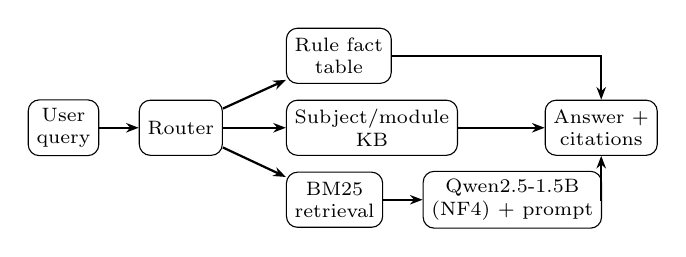
\begin{tikzpicture}[
  node distance=4mm and 5mm,
  box/.style={draw, rounded corners, align=center, minimum height=7mm, font=\scriptsize, inner sep=3pt},
  arr/.style={-{Stealth[length=1.6mm]}, thick}]
\node[box] (q) {User\\query};
\node[box, right=of q] (r) {Router};
\node[box, above right=2mm and 8mm of r] (f) {Rule fact\\table};
\node[box, right=8mm of r] (s) {Subject/module\\KB};
\node[box, below right=2mm and 8mm of r] (b) {BM25\\retrieval};
\node[box, right=of b] (l) {Qwen2.5-1.5B\\(NF4) + prompt};
\node[box, right=of s, xshift=6mm] (o) {Answer +\\citations};
\draw[arr] (q)--(r);
\draw[arr] (r)--(f);
\draw[arr] (r)--(s);
\draw[arr] (r)--(b);
\draw[arr] (b)--(l);
\draw[arr] (f.east)-|(o.north);
\draw[arr] (s)--(o);
\draw[arr] (l.east)-|(o.south);
\end{tikzpicture}
\caption{Routed query pipeline. Rule questions bypass the language model; free-text questions are answered only from retrieved passages, with a refusal path when retrieval is weak.}
\label{fig:arch}
\end{figure}

\subsection{Model configuration}
The generator is Qwen2.5-1.5B-Instruct loaded with 4-bit NF4 quantization (bitsandbytes) and float16 compute through Hugging Face Transformers and Accelerate, with automatic device mapping. Fact-bearing answers use greedy decoding (\texttt{do\_sample=False}); the prompt fixes the assistant persona and instructs it to answer only from the supplied context. The interface is a Gradio chat application.

\subsection{Knowledge base}
\label{sec:kb}
The knowledge base has two parts. The \emph{rules table} contains the regulations on passing criteria, attendance, grading and CGPA conversion. The \emph{subject table} contains, per course, its code, title, semester, category, credits, evaluation scheme, module-wise topics, textbooks and source. Every record stores \texttt{source\_url}, \texttt{fetched\_on} and a boolean \texttt{verified}. A record may be marked verified only if it carries an exact quotation from the fetched official document; values that could not be confirmed remain unverified and the assistant states this instead of guessing. A validator rejects records that violate these invariants. We enforced this policy after an early draft of the table contained a value that differed from the official regulations, which shows why such provenance is necessary.

\subsection{Document ingestion and retrieval}
Course material (PDF textbooks, slide decks, DOCX notes) is converted to text per page, slide or section, then split into chunks of about 800 characters with 120 characters of overlap, cut at sentence or paragraph boundaries. Each chunk carries its file, location and, when inferable from the file name, the subject code and module. Chunks are indexed with BM25. Subject-code tokens are kept intact and matched case-insensitively. Retrieval supports subject and module filters and returns nothing when the best score is below a configurable minimum, which implements the refusal path. Raw documents are third-party material and are not redistributed; only the ingestion code is published.

\section{Fine-tuning}
\subsection{Data}
Training pairs are generated from the knowledge base and chunks: rule questions, subject and module questions, passage-grounded questions with cited answers, and out-of-scope questions whose target answer is a refusal. Candidate pairs are filtered for length, duplicates and answer support (every factual claim must appear in the source passage), and a held-out split is created \emph{before} generation of training examples so that evaluation questions and their source passages do not appear in training.

\subsection{Procedure}
We apply QLoRA~\cite{dettmers2023qlora} to the 4-bit base model with low-rank adapters on the attention and MLP projection layers. Hyper-parameters (rank, scaling factor, learning rate, epochs, batch size) are fixed in the released training script and reported in Table~\ref{tab:hp} after the run. The adapter is small compared with the base model and can be loaded without modifying the base weights.

\begin{table}[t]
\caption{Fine-tuning configuration (values filled from the final run).}
\label{tab:hp}
\centering
\begin{tabular}{ll}
\toprule
Parameter & Value\\
\midrule
Base model & Qwen2.5-1.5B-Instruct\\
Quantization & 4-bit NF4, fp16 compute\\
LoRA rank / alpha / dropout & \tbd\\
Learning rate / schedule & \tbd\\
Epochs / effective batch size & \tbd\\
Training examples / held-out examples & \tbd\\
Hardware / wall-clock time & \tbd\\
\bottomrule
\end{tabular}
\end{table}

\section{Evaluation Protocol}
We evaluate four configurations on the same held-out set: (A) the base model with only the system prompt, (B) the base model with retrieval, (C) the fine-tuned model without retrieval, and (D) the full system (fine-tuned model with routing and retrieval). The question set contains four groups: university-rule questions, subject and module questions, passage-grounded textbook questions, and out-of-scope questions that should be refused. We report:
\begin{itemize}
\item \textbf{Fact exact-match:} the fraction of rule questions whose answer contains the correct value.
\item \textbf{Hit@$k$:} whether the gold passage is among the top-$k$ retrieved chunks.
\item \textbf{Citation correctness:} whether every cited file and page supports the sentence it is attached to, judged against the source.
\item \textbf{Refusal accuracy:} the fraction of out-of-scope questions correctly refused, and the false-refusal rate on in-scope questions.
\end{itemize}
Generation is greedy so results are reproducible for a fixed model and index.

\section{Results}
\label{sec:results}
Results are pending completion of the final training run.

\begin{table}[t]
\caption{Held-out evaluation (to be completed from \texttt{eval/results.json}).}
\label{tab:results}
\centering
\begin{tabular}{lcccc}
\toprule
Config. & Fact EM & Hit@5 & Cite. & Refusal\\
\midrule
A: base + prompt & \tbd & \tbd & \tbd & \tbd\\
B: base + retrieval & \tbd & \tbd & \tbd & \tbd\\
C: fine-tuned only & \tbd & \tbd & \tbd & \tbd\\
D: full system & \tbd & \tbd & \tbd & \tbd\\
\bottomrule
\end{tabular}
\end{table}

\section{Discussion and Limitations}
Rule answers are deterministic and therefore as correct as the underlying table, which is why the table carries provenance. The model's free-text answers remain subject to the usual limits of a 1.5B-parameter generator: it may paraphrase a passage inexactly, so citations are shown to let the student check the source. Coverage is limited to the courses and semesters whose official syllabus text could be verified, and the system says so for others. Fine-tuning data are synthetic, so the evaluation set should be extended with questions written by students and faculty. The prototype runs on a hosted GPU session and downloads the model weights on first use; it is not an offline system unless the weights are stored locally and the public share link is disabled.

\section{Conclusion}
Campus GPT demonstrates a grounded design for a university assistant built on a small, quantized language model: deterministic answers for rules, structured data for subjects, retrieval with citations for course material, and refusal when evidence is missing. The released pipeline allows the knowledge base to be extended to more branches and schemes. Future work includes multilingual and voice interfaces, mock tests and quizzes, and dense retrieval as an optional second stage.

\section*{Acknowledgment}
The authors thank the Department of Artificial Intelligence and Machine Learning, Acharya Institute of Technology, for support.

\begin{thebibliography}{00}
\bibitem{lewis2020rag} P.~Lewis \textit{et al.}, ``Retrieval-augmented generation for knowledge-intensive NLP tasks,'' in \textit{Advances in Neural Information Processing Systems (NeurIPS)}, vol.~33, 2020, pp.~9459--9474.
\bibitem{robertson2009bm25} S.~Robertson and H.~Zaragoza, ``The probabilistic relevance framework: BM25 and beyond,'' \textit{Foundations and Trends in Information Retrieval}, vol.~3, no.~4, pp.~333--389, 2009.
\bibitem{hu2022lora} E.~J. Hu \textit{et al.}, ``LoRA: Low-rank adaptation of large language models,'' in \textit{Proc.\ Int.\ Conf.\ Learning Representations (ICLR)}, 2022.
\bibitem{dettmers2023qlora} T.~Dettmers, A.~Pagnoni, A.~Holtzman, and L.~Zettlemoyer, ``QLoRA: Efficient finetuning of quantized LLMs,'' in \textit{Advances in Neural Information Processing Systems (NeurIPS)}, vol.~36, 2023.
\bibitem{qwen2025} A.~Yang \textit{et al.}, ``Qwen2.5 technical report,'' arXiv:2412.15115, 2024.
\bibitem{sanh2019distilbert} V.~Sanh, L.~Debut, J.~Chaumond, and T.~Wolf, ``DistilBERT, a distilled version of BERT: smaller, faster, cheaper and lighter,'' arXiv:1910.01108, 2019.
\end{thebibliography}

\end{document}
